\documentclass{beamer} 
\usepackage{amsmath,amsthm}
\usepackage{graphicx,microtype,parskip}
\usepackage{caption,subcaption,multirow}
\usepackage{attrib}

\frenchspacing

\usetheme{default}
\usecolortheme{whale}

\setbeamertemplate{navigation symbols}{}

\setbeamercolor{title}{fg=blue,bg=white}

\setbeamercolor{block title}{fg=white,bg=gray}
\setbeamercolor{block body}{fg=black,bg=lightgray}

\setbeamercolor{block title alerted}{fg=white,bg=darkgray}
\setbeamercolor{block body alerted}{fg=black,bg=lightgray}

\AtBeginSection[]
{
  \begin{frame}
    \tableofcontents[currentsection]
  \end{frame}
}


\title{Gambling with Australian brachiopods}
\author{Peter D Smits}
\institute{Committee on Evolutionary Biology, University of Chicago}

\begin{document}

\begin{frame}
  \maketitle
\end{frame}

\begin{frame}
  \frametitle{Foundation}

  \begin{alertblock}{Question}
    Why do taxa go extinct at different rates?
  \end{alertblock}
\end{frame}


\begin{frame}
  \frametitle{Common observation}

  \begin{block}{Pattern}
    Species with large geographic ranges have a low extinction risk.
  \end{block}

  \bigskip

  \begin{center}
    Expected given \alert{purely random} extinction.
  \end{center}
\end{frame}


\begin{frame}
  \frametitle{Gambler's Ruin}

  \begin{definition}
    Given infinite time, all gambler's go bust. 
  \end{definition}
\end{frame}


\begin{frame}
  \frametitle{Same rates}

  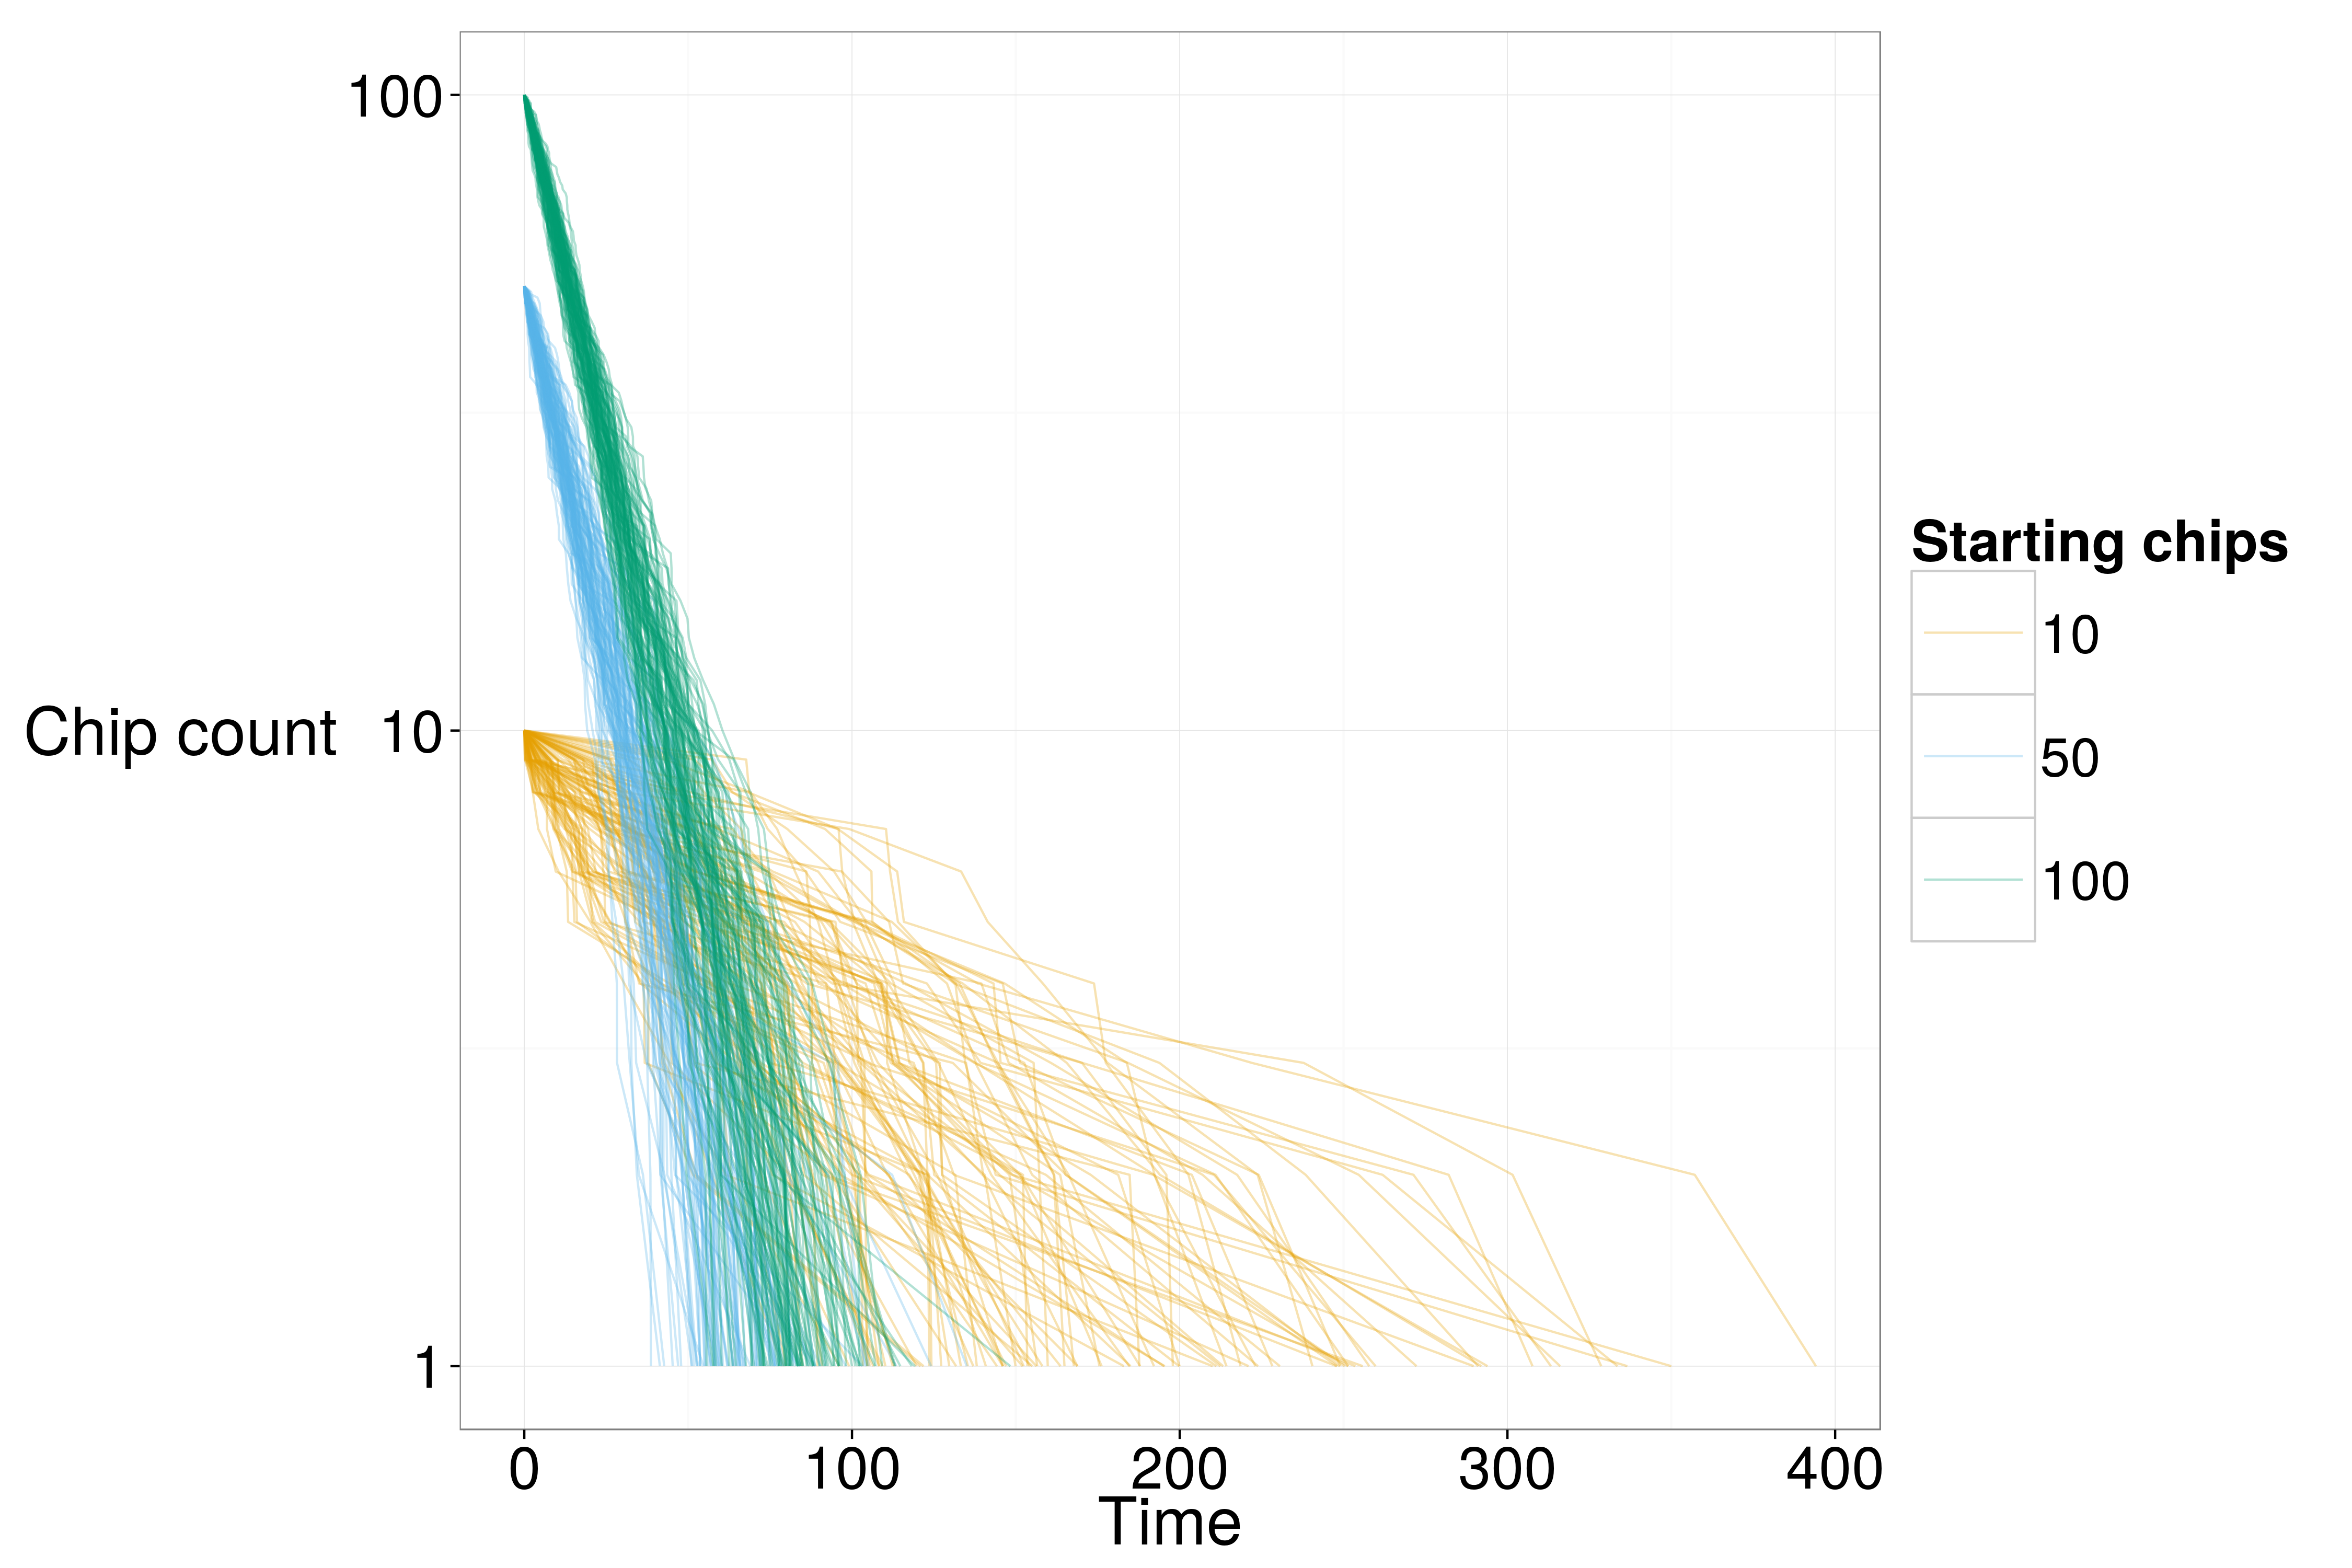
\includegraphics[width = \textwidth, height = 0.8\textheight, keepaspectratio = true]{figure/gambling}
\end{frame}


\begin{frame}
  \frametitle{Different rates}

  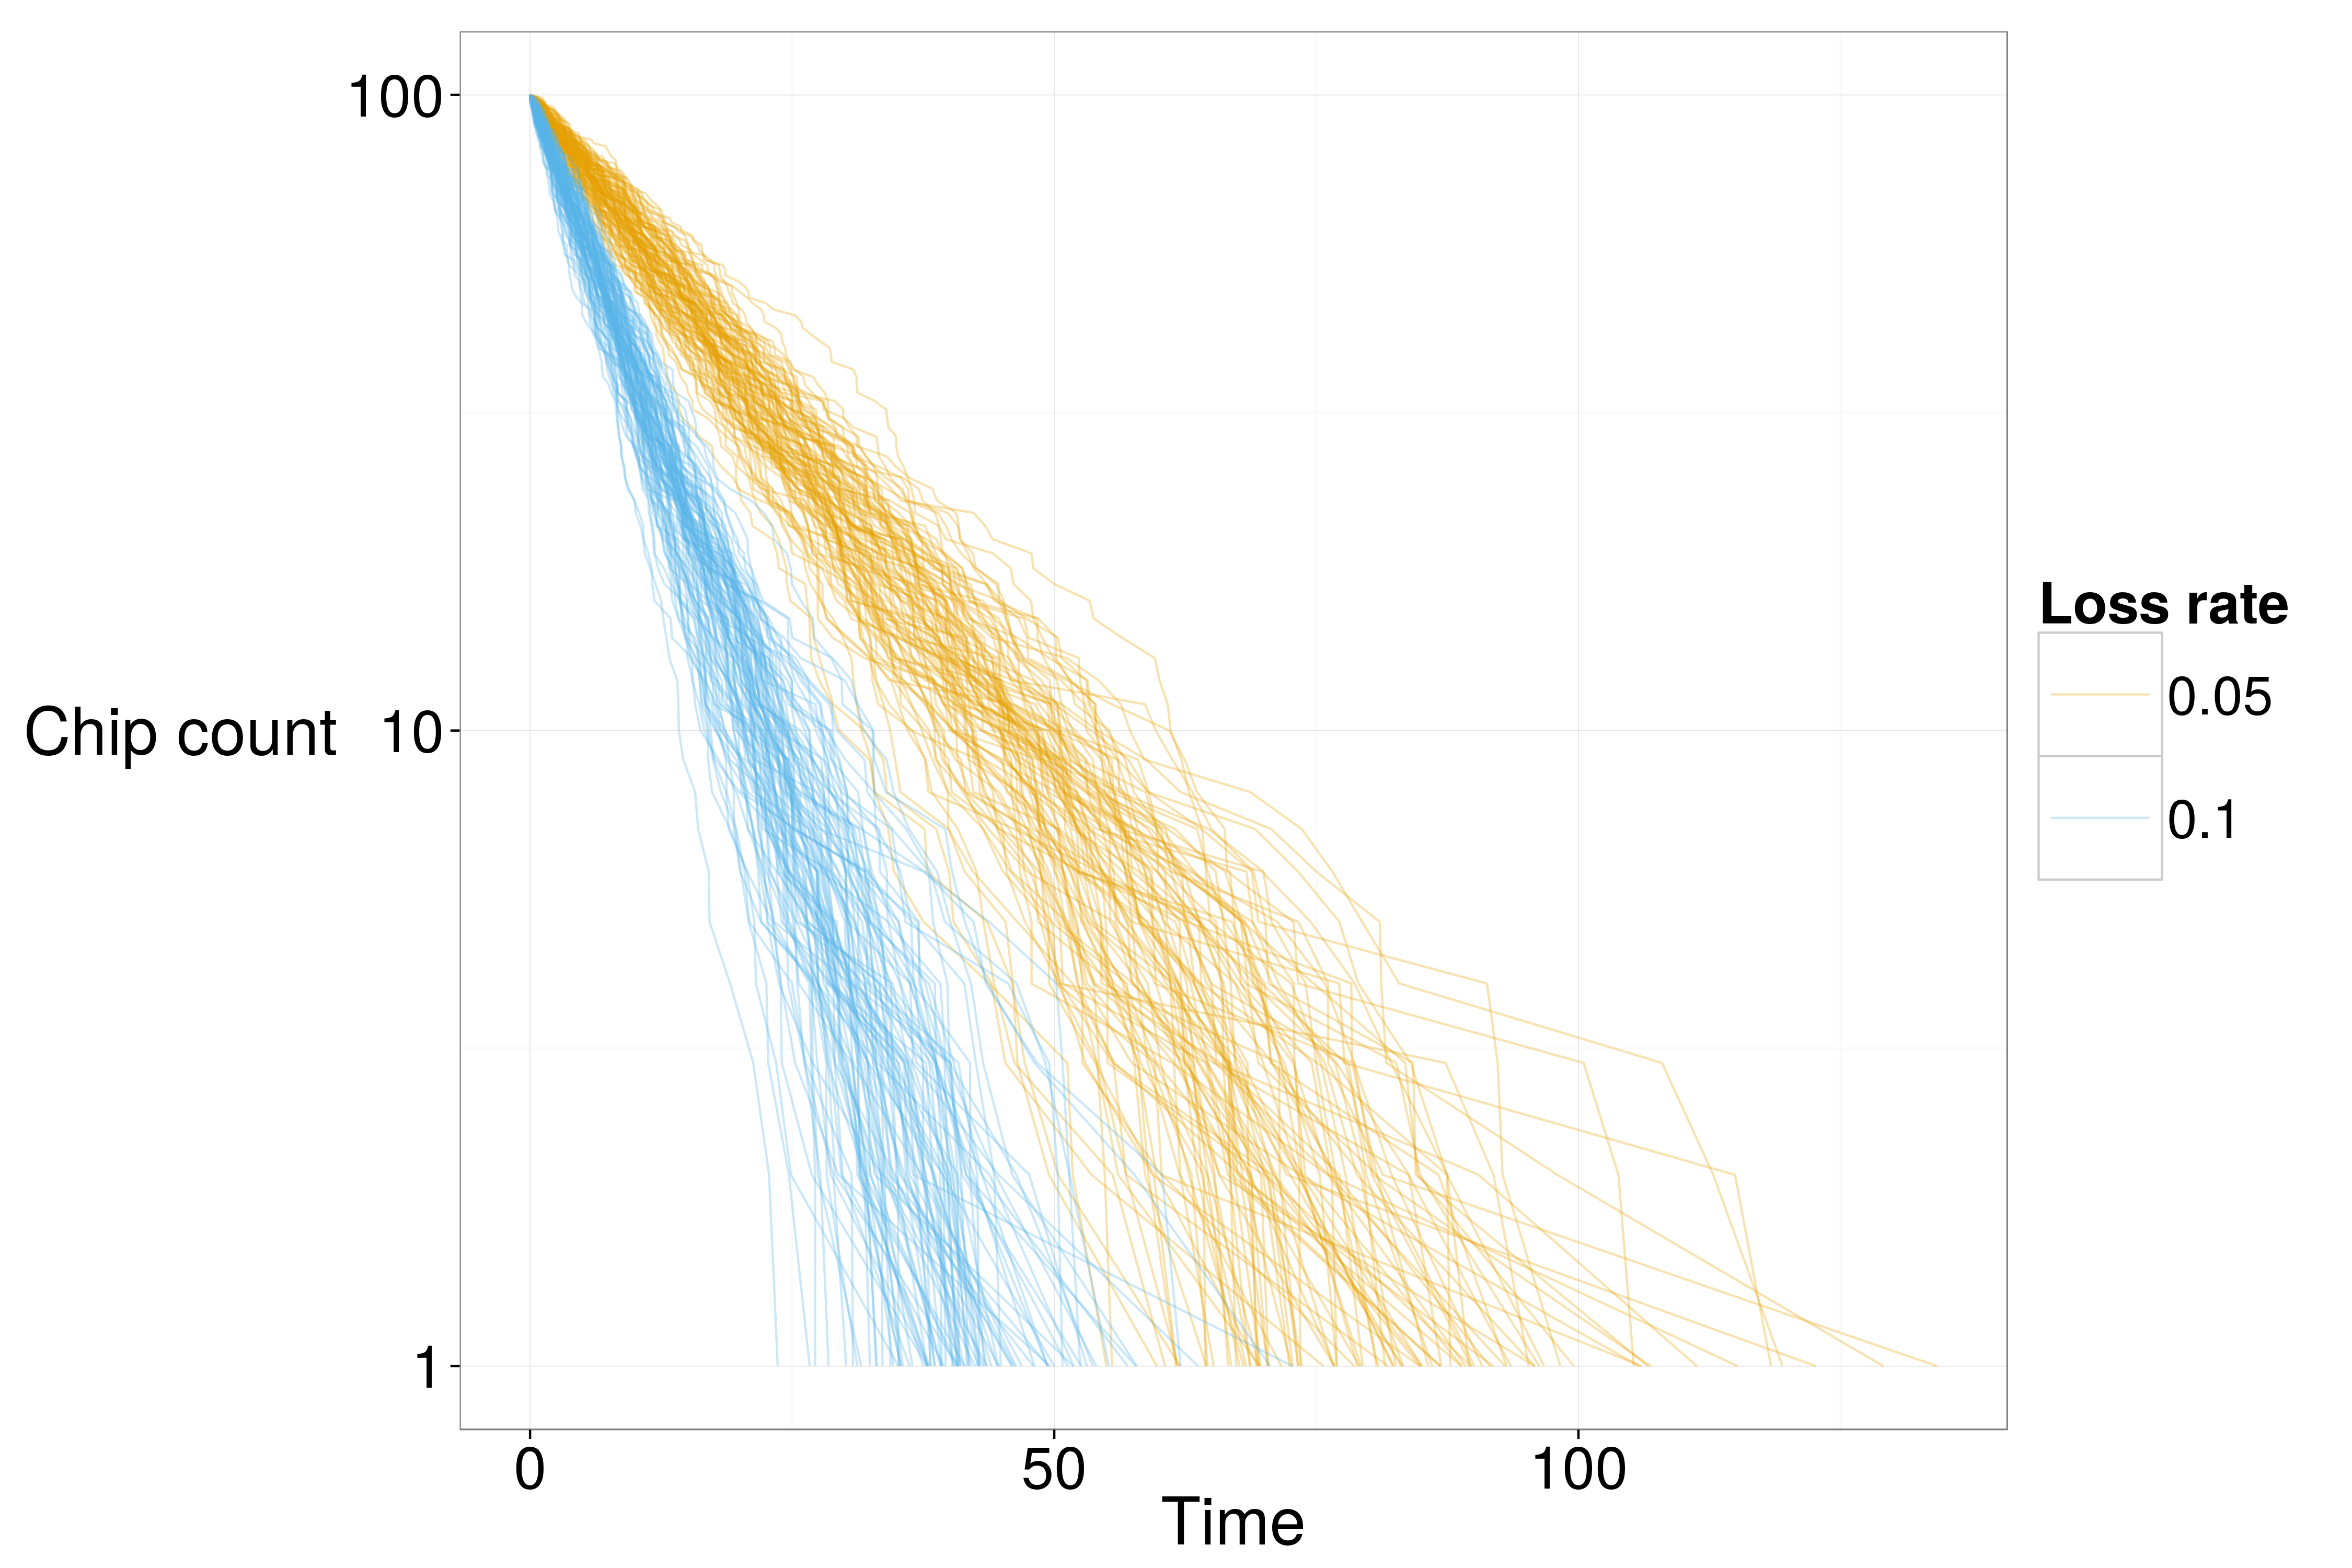
\includegraphics[width = \textwidth, height = 0.8\textheight, keepaspectratio = true]{figure/gsame}
\end{frame}


\begin{frame}
  \frametitle{Mechanism}
  \begin{alertblock}{Problem}
    Impossible to distinguish \alert{random} from \alert{selection} without more information.
  \end{alertblock}
\end{frame}


% Ecology and interactions with the environment
\begin{frame}
  \frametitle{Adaptive zones}

  \begin{center}
    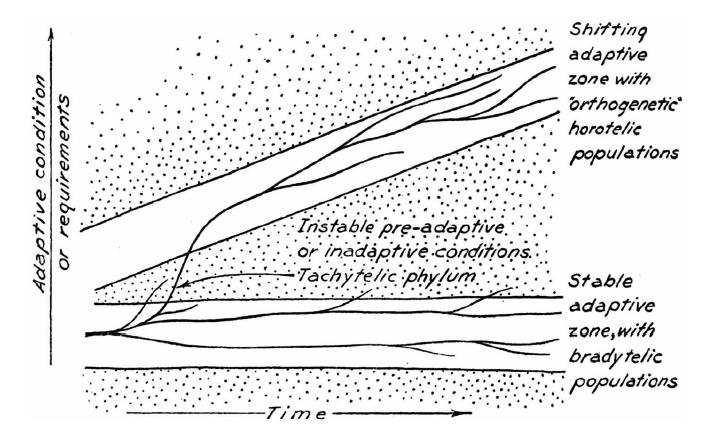
\includegraphics[height = 0.7\textheight, keepaspectratio = true]{figure/simpson}

    \tiny{\attrib{Simpson 1944 \underline{Tempo and Mode}}}
  \end{center}
\end{frame}

% Enter Brachiopods
\begin{frame}
  \frametitle{Enter brachiopods}

  Permian

  Australia and New Zealand (pbdb + fred)

  substrate affinity

  paleoenvironment affinity
\end{frame}


\begin{frame}
  \frametitle{Brachiopods, environmental preference, and extinction}

  \begin{alertblock}{Question}
    Do interactions involved in environmental preference predict differential survival?
  \end{alertblock}
\end{frame}

\begin{frame}
  \frametitle{Formalization of Van Valen}

  \begin{block}{Law of Constant Extinction}
    \begin{columns}
      \begin{column}{0.5\textwidth}
        \begin{align*}
          T &\sim Exp(\lambda)\ \\ 
          &\sim Weibull(\lambda, k = 1) 
        \end{align*}
      \end{column}
      \begin{column}{0.5\textwidth}

        \(T\): survival time
        
        \(\lambda\): expected number of \\extinctions per unit time
        
        \(k\): time proportionality
      \end{column}
    \end{columns}

  \end{block}
\end{frame}


% Preliminary analytical framework


% Results


% Future modeling
\begin{frame}
  \frametitle{Bayesian framework}

  better capture uncertainty

  continuous model development

  interpretability 

\end{frame}


\begin{frame}
  \frametitle{Affinity is a distribution, not a scalar}

  e.g. Pr(taxon carbonate draw \(\mid\) all taxon draw) has uncertainty.

  Improved prior e.g. substrate affinity:
  \begin{align*}
    (\theta_{\text{carb}} \mid \text{rocks}) &\sim Bin(\text{carb} \mid \text{rocks}, \theta_{\text{carb}}) Beta(\alpha, \beta) \\
    &\sim Beta(\text{carb} + \alpha, \text{rocks} - \text{carb} + \beta)
  \end{align*}

  Estimate affinity as part of model. 
  
  Propagate uncertainty.

\end{frame}


\begin{frame}
  \frametitle{Acknowledgements}
  \begin{columns}
    \begin{column}{0.5\textwidth}
      \begin{itemize}
        \item Advising
          \begin{itemize}
            \item Kenneth D. Angielczyk, Michael J. Foote
            \item P. David Polly, \\Richard H. Ree
          \end{itemize}

        \item Discussion and advice
          \begin{itemize}
            \item David Bapst, Megan Boatright, Ben Frable, Marites Villarosa Garcia, Kathleen Ritterbush, Darcy Ross, Liz Sander, Carl Simpson
          \end{itemize}
      \end{itemize}
    \end{column}
    \begin{column}{0.5\textwidth}
      
\includegraphics[height = 0.3\textheight, keepaspectratio = true]{figure/chicago} 
      
\includegraphics[width = 0.4\textwidth, keepaspectratio = true]{figure/field}

      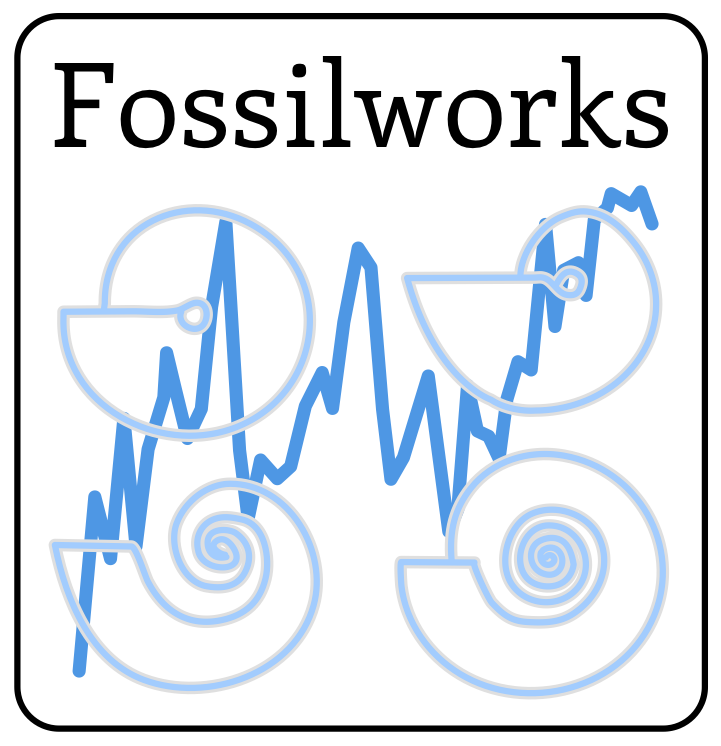
\includegraphics[height = 0.3\textheight, width = 0.5\textwidth, keepaspectratio = true]{figure/fossilworks}
      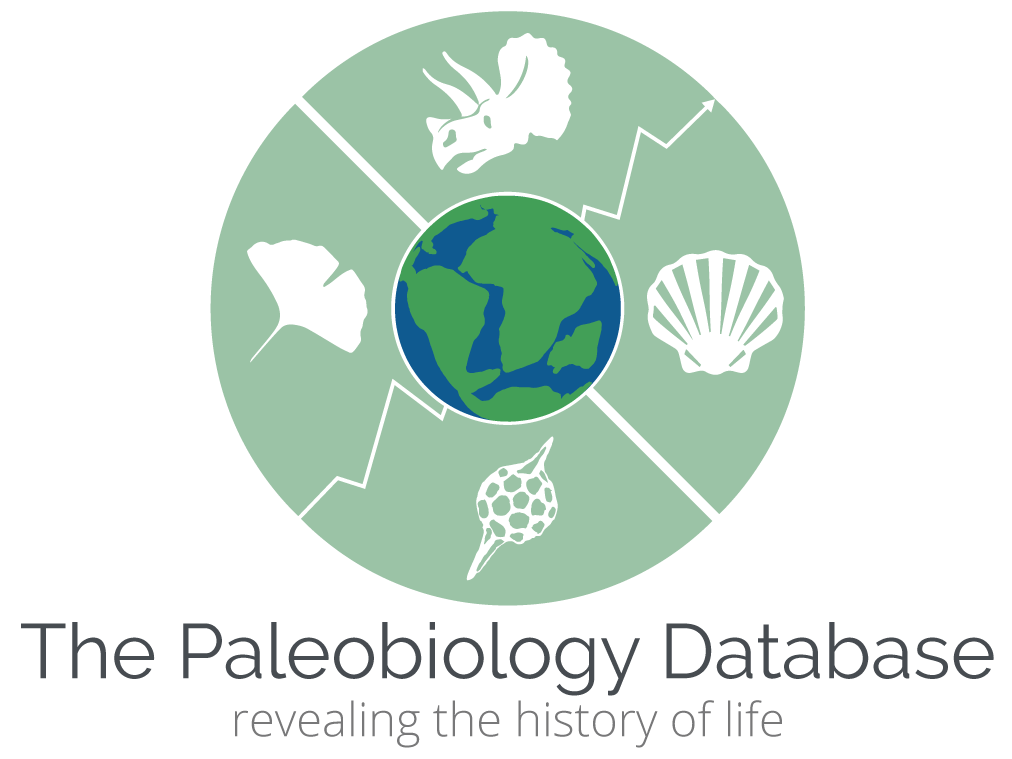
\includegraphics[width = 0.5\textwidth, keepaspectratio = true]{figure/paleodb}

    \end{column}
  \end{columns}
\end{frame}


\end{document}
